\documentclass[11pt]{article}
\usepackage{amsthm}
\usepackage{amsmath}
\usepackage{amssymb}
\usepackage[spanish,es-tabla]{babel}
%\usepackage[style=numeric,sorting=none]{biblatex}
\usepackage{bm}
\usepackage{booktabs}
\usepackage{enumitem}
\usepackage{fancyhdr}
\usepackage{float}
\usepackage[utf8]{inputenc}
\usepackage{listingsutf8}
\usepackage[top=2.5cm,bottom=2.5cm,left=2.5cm,right=2.5cm]{geometry}
\usepackage{graphicx}
\usepackage{hyperref}
\usepackage{longtable}
\usepackage{multicol}
%\usepackage{subcaption}
\usepackage{subcaption}
\usepackage{svg}
\usepackage{verbatim}
\usepackage{xcolor}
\usepackage{xstring}

\definecolor{codegreen}{rgb}{0,0.6,0}
\definecolor{codegray}{rgb}{0.5,0.5,0.5}
\definecolor{codepurple}{rgb}{0.58,0,0.82}
\definecolor{backcolour}{rgb}{0.99,0.995,0.99}

\lstdefinestyle{mystyle}{
    backgroundcolor=\color{backcolour},   
    commentstyle=\color{codegreen},
    keywordstyle=\color{magenta},
    numberstyle=\tiny\color{codegray},
    stringstyle=\color{codepurple},
    basicstyle=\ttfamily\small,
    breakatwhitespace=false,         
    breaklines=true,                 
    captionpos=b,                    
    keepspaces=true,                 
    numbers=left,                    
    numbersep=5pt,                  
    showspaces=false,                
    showstringspaces=false,
    showtabs=false,                  
    tabsize=2
}
%\label{ tab: \StrBefore{#1}{.} } 

\newcommand{\figura}[3]{\begin{figure}[H] \centering \includegraphics[#3]{#1} \caption{#2} \label{#1}  \end{figure}}
\newcommand{\tablasimple}[2]{\begin{table}[H] \centering \input{#1} \caption{#2} \label{#1} \end{table}}
\newcommand{\tablalarga}[2]{ \begin{center} \input{#1} \begin{table}[H] \caption{#2} \label{#1} \end{table} \end{center}}

\lstset{style=mystyle}
\decimalpoint
% Adding references
% \addbibresource{../../referencias.bib}
% Auxiliar commands
\newcommand{\work}{Proyecto Final: Redes Neuronales}
% Changes space between lines of equations
\setlength{\jot}{10pt}
% Changes space between text and equations
\setlength{\abovedisplayskip}{100pt}
\setlength{\belowdisplayskip}{100pt}
\setlength{\abovedisplayshortskip}{100pt}
\setlength{\belowdisplayshortskip}{100pt}
% Theorem environment in case I need it
\newtheorem{theorem}{Teorema}
% make header
\pagestyle{fancy}
\fancyhf{}
\vspace{1cm}
\rhead{}
\lhead{\work}
\cfoot{\thepage}
%  Text info
\title{\textbf{\work}}
\author{Curso Avanzado de Estadística. Profa. Guillermina Eslava Gómez.\\ \\ Aldo Sayeg Pasos Trejo. César Cossio Guerrero. \\ \\ Posgrado en Ciencias Matemáticas. Universidad Nacional Autónoma de México. }
\date{\today}
\begin{document}
\maketitle
\section{Introducción}
El trabajo consistió en ajustar una regresión logística y varios modelos de redes neuronales con la finalidad de clasificar dígitos escritos a mano correspondientes a la base de datos de MNIST. En el Anexo 1 a este trabajo se puede encontrar un breve análisis exploratorio de la base de datos. Para los modelos de redes neuronales, los modelos se entrenaron optimizando la función de pérdida dada por la entropía categórica. %, que está definida por la ecuación:
%\begin{equation}
%    L(\bm{y},\bm{\hat{y}}) = - \sum_{i=0}^{9} y_i \ln{(\hat{y}_{i})}
%\end{equation}
\\
\\Se escogió dicha función de pérdida ya que, además de ser considerada un estándar para la clasificación entre grupos, es la función que presenta mejor estabilidad a la hora de entrenar los modelos y no presupone nada sobre la distribución de las clases. La regresión logística se optimizó minimizando esa misma función. Para tanto las redes neuronales como para la regresión logística los ajustes se realizaron sobre la base de datos estandarizada para que la variable correspondiente a cada pixel tuviera error estándar 1 y promedio 0.
\\
\\En el presente trabajo, se ajustó solo una regresión logísitca sobre todas las variables y se comparó con seis redes neuronales multicapa (``Deep Neural Networks'', DNN) y seis redes neuronales multicapa convolucionales sobre las imágenes (``Convolutional Neural Networks'', CNN), para un total de 12 redes neuronales. La decisión de utilizar también redes convolucionales se tomó debido a que sabemos que los datos corresponden a imágenes, no solo a variables numéricas, y existe una basta literatura sobre como los filtros convolucionales y otra clase de herramientas de procesamiento digital de imágenes nos permiten mejorar las tasas de error de los clasificadores de una manera sustancial \cite{lecunn,Ripley}.
\\
\\Los modelos de redes neuronales se ajustaron con la librería Tensor Flow, utilizando las herramientas de Keras \cite{tf}. Como la gran mayoría de los softwares para redes neuronales, este programa utiliza una versión modificada del algoritmo de descenso de gradiente estocástico (SGD) para optimizar la función de pérdida. Dicho algoritmo, el algoritmo ADAM, básicamente es una versión pesada del SGD para evitar los mínimos locales.  Uno de los hiperparámetros más importantes para el SGD y, por lo tanto para ADAM, es el tamaño del ``batch size''. El ``batch size'' es el número de observaciones, tomadas aleatoriamente de la muestra original, con el que se calcula el gradiente en cada iteración del algoritmo. El batch size es inversamente proporcional al número de pasos de optimización que contiene una época de optimización. Así, es claro que a menor batch size habrá más pasos de optimización. Aunque en principio eso motiva a tomar un batch size muy pequeño, los análisis muestran que en muchas ocasiones tomar un batch size mayor reduce las épocas necesarias para entrenar. Se realizó un análisis para encontrar un batch size óptimo, como muestran las figuras \ref{fig:bsError} y \ref{fig:bsLoss}.
\begin{figure}[h]
    \centering
    \begin{subfigure}[c]{0.40\textwidth}
        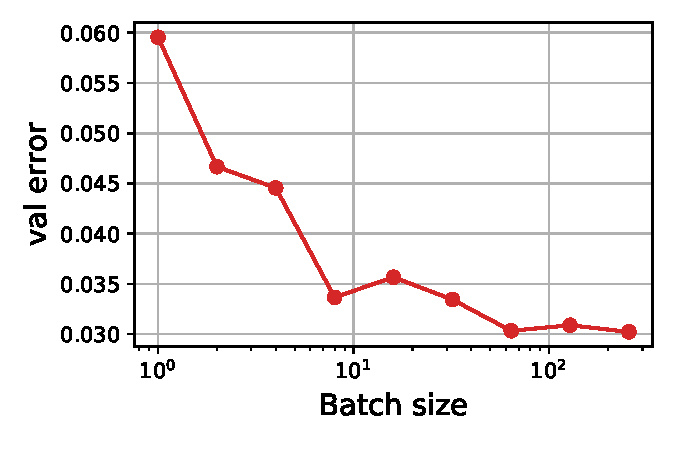
\includegraphics[width=\textwidth]{batchSizeAnalError.pdf}
        \caption{}
        \label{fig:bsError}
    \end{subfigure}
    \begin{subfigure}[c]{0.4\textwidth}
        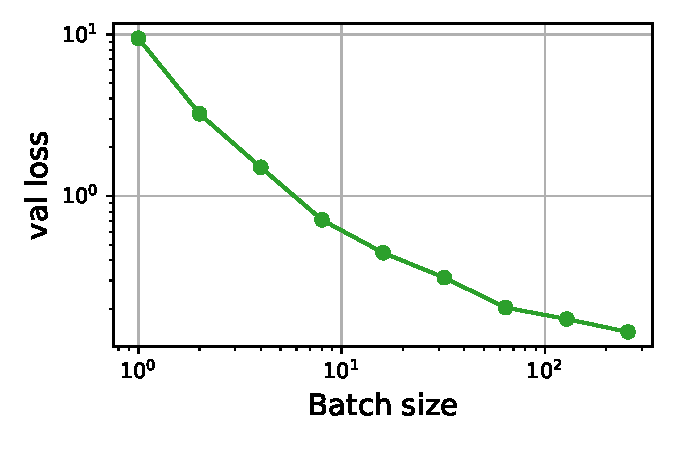
\includegraphics[width=\textwidth]{batchSizeAnalLoss.pdf}
        \caption{}
        \label{fig:bsLoss}
    \end{subfigure}
    \caption{Error y funcion de perdida como función del batch size. El error se presenta en tasa}
\end{figure}
La mínima tasa de error se encuentra para el valor de 256. Sin embargo, con ese valor se encontró que algunos sistemas eran muy sensibles a las condiciones iniciales a la hora de realizar validación cruzada y se atascaban en mínimos locales. Así, se prefirió tomar como valor de batch size 128, que presentaba mayor estabilidad.
\section{Regresión Logística}
Para el ajuste de regresión logística multinomial, no se realizó regularización alguna sobre el ajuste. A su vez, por ser un problema en el que no hay una clase que podamos tomar naturalmente como clase de referencia, el ajuste se realizó sin tomar una clase de referencia, que se puede interpretar como una regresión lineal para el logit de cada probabilidad. Se obtuvieron las tasas de error mostradas en la tabla \ref{tab:logreg}
\begin{table}[H]
    \centering
    \begin{tabular}{c|c|c|c}
        \toprule
        error & val error & cv val error mean & cv val error std \\
        \midrule
        6.0500 &  7.8000 & 7.7650 & 0.1977  \\
        \bottomrule
    \end{tabular}
    \caption{Porcentajes de error para la regresión logística. Los errores de validación cruzada se obtuvieron para $k=5$ folds y una sola repetición.}
    \label{tab:logreg}
\end{table}
La validación cruzada realizó de manera estratificada, es decir, procurando que cada fold mantuviera la misma proporción entre clases que el conjunto de entrenamiento original. La regresión logística tuvo un tiempo de ejecución muy alto, tardando alrededor de 2.7 horas de cómputo aún distribuyendo el proceso entre distintos núcleos de procesador. Un tiempo de cómputo tan alto nos impide realizar más iteraciones del proceso de validación cruzada en un tiempo aceptable.
\section{Modelos DNN}
Para trabajar con los modelos de redes neuronales densas, primero exploramos algunas posibilidades en sus funciones de activación, cuyos distintos perfiles se muestran en la siguiente figura:
\figura{activations.pdf}{Algunas funciones de activación integradas en el software Tensor Flow.}{width = 0.5\textwidth}
Si todas las capas ocultas de la red tienen funciones de activación lineales, la red es equivalente a una regresión logística \cite{Goodfellow}. Así, un hiperparámetro importante es la función de activación de una capa. A su vez, el número de capas necesarias para la red puede ser cuestión de controversia, ya que a mayor número de capas es posible que el modelo necesite muchas más épocas para entrenarse y sea más suceptible a entrar en mínimos locales. Sin emabargo, el número de parámetros entrenables puede disminuir considerablemente al agregar capas de tamaño pequeño.
\\
\\Los pesos de cada arista y las constantes de cada nodo se pueden regularizar. Otro parámetro signficativo son las capas de Dropout, las cuales seleccionan aleatoriamente una fracción de aristas entre dos capas y vuelven su peso 0. Dichas capas se pueden interpretar como una especie de regularización sobre los pesos del modelo, y por lo general ayudan al modelo a tener una mejor generalización en la predicción.
\\
\\Debido a las amplias posiblidades existentes para seleccionar hiperparámetros, es difícil realizar una selección de modelos estructurada, por lo que se recurrió a un método de búsqueda aleatoria entre los hiperparámetros de los modelos. En general, se observó que para pocos nodos en la primera capa (menos de 200), el valor óptimo para el Dropout de entrada era de 0.2, mientras que para muchos nodos en la primera capa era preferible utilizar un valor más grande.
\\
\\La tangente hiperbólica resultó ser la mejor función para las capas, al igual que la función swish, que parece una versión suavizada de la función de activación lineal rectificada. Después de dichos procesos de experimentación, los modelos seleccionados con menores tasas de error de validación se muestran en la tabla \ref{tab:DNNdes}.
\begin{table}[H]
    \centering
    \begin{tabular}{c| p{1.5cm}| p{1cm}| p{2cm}| p{3.5cm}| p{2.5cm} | p{1.5cm}| p{1cm}}
        \toprule
        Name &  Trainable Parameters &  Dense Layers & Nodes per Layer &  Activation Functions &  Regularization & Dropout & Input Dropout \\
        \midrule
        DNN1 &  318010 & 1 & [400] & [tanh] & [0] & [0.1] & 0.5 \\
        DNN2 &  178110 & 2 & [200, 100] & [tanh, swish] & [0.005,0.001] & [0,0] & 0.2 \\
        DNN3 &  178110 & 2 & [200, 100] & [tanh, tanh] & [0.005,0.001] & [0,0] & 0.2 \\
        DNN4 &  188210 & 3 & [200, 100, 100] & [tanh, tanh, tanh] & [0.001, 0,0] & [0,0,0] & 0.2 \\
        DNN5 &  203260 & 3 & [200, 150, 100] & [tanh, relu, tanh] & [0.001, 0,0] & [0,0,0] & 0.2 \\
        DNN6 &  213360 & 4 & [200, 150, 100, 100] & [tanh, swish, tanh, swish] & [0.001, 0,0,0] & [0,0,0,0] & 0.2 \\
        \bottomrule
    \end{tabular}
    \caption{Descripción de los seis modelos DNN. La columna Dropout indica el valor del dropout después de la capa densa. Input Dropout es la fracción de dropout entre la entrada de datos y la primera capa densa. La columna Regularization indica la regularización sobre las aristas posteriores a cada capa densa.}
    \label{tab:DNNdes}
\end{table}
Los modelos pueden visualizarse esquemáticamente en las figuras \ref{fig:DNN1}, \ref{fig:DNN2}, \ref{fig:DNN3}, \ref{fig:DNN4}, \ref{fig:DNN5} y \ref{fig:DNN6}, contenidas en el Anexo 4 de nuestro trabajo. Los modelos se entrenaron durante 100 épocas y se realizó validación cruzada con $k=10$ folds y una sola repetición. Los resultados de dicho procedimiento se muestran en la tabla \ref{tab:DNNres}.
\begin{table}[H]
    \centering
    \begin{tabular}{c| p{1.5cm}| p{1.5cm}| p{1.5cm}| p{1.5cm}| p{1.5cm}| p{1.5cm}| p{1.5cm}| p{1.5cm}}
        \toprule
        Name &  error &  val error &  cv val error mean &  cv val error std &  loss &  val loss &  cv val loss mean &  cv val loss std \\
        \midrule
        DNN1 &  1.935 &      2.367 &              4.930 &             0.256 & 0.058 &     0.104 &             0.159 &            0.010 \\
        DNN2 &  0.000 &      2.444 &              2.997 &             0.382 & 0.000 &     0.342 &             0.662 &            0.156 \\
        DNN3 &  0.972 &      2.633 &              3.380 &             0.169 & 0.033 &     0.193 &             0.161 &            0.013 \\
        DNN4 &  1.342 &      2.622 &              8.470 &             0.544 & 0.355 &     0.390 &             1.351 &            0.050 \\
        DNN5 &  1.152 &      2.544 &              8.077 &             0.609 & 0.368 &     0.432 &             1.336 &            0.031 \\
        DNN6 &  1.050 &      2.533 &              8.055 &             0.899 & 0.358 &     0.406 &             1.366 &            0.040 \\
        \bottomrule
        \end{tabular}
        \caption{Errores y función de pérdida para las redes DNN. Los errores se muestran en porcentaje}
        \label{tab:DNNres}
\end{table}
\section{Modelos CNN}
Como ya se mencionó, se entrenaron 6 modelos que hacen uso de capas de convolución. En el anexo 2 de este trabajo se puede encontrar una breve explicación de su funcionamiento. Ahora bien, la exploración que realizamos estuvo principalmente enfocada en optimizar la precisión y las tasas de error de los siguientes aspectos de un modelo CNN: el número de capas convolucionales (capa Convolucional + Capa Max Pool), el número de filtros que cada uno de los bloques generan, el valor de Dropout previo a la primer capa densa, el tamaño del kernel de la capa de convolución, el tamaño de \textit{stride}, el uso de \textit{Padding}, la efectividad del uso de Batch Normalization y de Data Augmentation. Estos son los aspectos básicos de una CNN,  y decidimos no explorar más hiperparámetros por falta de recursos computacionales. 
\\
\\
La figura \ref{fig:6Graf}, contenida en el Anexo 4 del presente trabajo, nos indica cómo se seleccionaron los hiperparámetros para estos modelos. Primero, de la subfigura \ref{fig:DropOut} seleccionamos el valor de $0.5$ para el Dropout; mientras que con base en las subfiguras \ref{fig:FCNodes}, \ref{fig:FullConn2CL} y \ref{fig:FullConn3CL}, escogimos el valor de 100 nodos para todas las capas densas. Si bien cada modelo tiene número de nodos óptimos para la capa densa, la diferencia en precisión respecto del valor que se obtiene con $100$ nodos es pequeño. A partir de los experimentos resumidos en la figura \ref{fig:KernelSize}, seleccionamos el número de filtros como $32$, $64$, $128$ para la primera, segunda y tercera capa de convolución, respectivamente; para terminar, basándonos en la subfigura \ref{fig:ConvNodes} seleccionamos el tamaño del kernel de las capas de convolución como $3x3$.
\\
\\
En cuanto a la selección de la arquitectura de las capas de convolución, podemos abordar cada operación y su importancia. En primer lugar, Batch Normalization se encarga de reescalar los valores de salida de las capas y se piensa que mejora la precisión de los resultados. En segundo lugar, Data Augmentation genera imágenes de manera aleatoria con base en ciertas operaciones sobre las imágenes originales, como rotaciones, traslaciones, zoom, entre otras; con lo cual se aumenta el conjunto de datos original y se fomenta la generalización del modelo. El uso de Padding está asociado con no perder información relevante en las orillas de las imagenes. Como no conocemos cada una de las imágenes es que se decidió utilizar para conservar toda la información. En cuarto lugar, se decidió utilizar Stride como un parámetro fijo (igual a 1) para mantener la mayor información posible, al costo de que esta este altamente correlacionada. En quinto lugar, se decidió utilizar la función de activación RELU pues experimentalmente observamos que mantuvo un buen funcionamiento a comparación de otras. 
\\
\\Cabe destacar que, para la selección de hiperparámetros, también se consideraron otros aspectos que no fueron puramente debidos a la optimización de parámetros o por cuestiones computacionales, sino que fue por estudiar arquitecturas que ha mostrado dar buenos resultados como: \textit{VGG16}, \textit{InceptionV}, \textit{ResNet}, \textit{AlexNet}  entre otras.
\\
\\Con base en el análisis de dichos parámetros, se seleccionaron los 6 modelos mostrados en la tabla \ref{tab:CNNdes}. 
\begin{table}[H]
    \centering
    \begin{tabular}{c| p{1.5cm}| p{1.5cm}| p{1.5cm}| p{1.5cm}|  p{1.5cm}|  p{2.2
    cm} | p{1.5cm} | p{1.5cm}}
        \toprule
        Name &  Trainable Parameters &  Dense Layers &  Conv. Layers &  Nodes per Layer & Activation Functions &  Regularization & Dropout & Input Dropout \\
        \midrule
        CNN1 & 542230 & 1 & 1 &  [100] & [relu] & [0] & [0] & [0] \\
        CNN2 & 542230 & 1 & 1 &  [100] & [relu] & [0] & [0] & [0.5] \\
        CNN3 & 179926 & 1 & 2 &  [100] & [relu] & [0] & [0] & [0] \\
        CNN4 & 180118 & 1 & 2 &  [100] & [relu] & [0] & [0] & [0.5] \\
        CNN5 & 209430 & 1 & 3 &  [100] & [relu] & [0] & [0] & [0] \\
        CNN6 & 209430 & 1 & 3 &  [100] & [relu] & [0] & [0] & [0] \\
        \bottomrule
    \end{tabular}        
    \caption{Descripción sintetizada de los modelos de redes convolucionales}
    \label{tab:CNNdes}
\end{table}
Para la descripción de la parte de convolución, la tabla \ref{tab:CNNconvDes} describe la arquitectura de las capas de convolución usando la nomenclatura de la tabla \ref{tab:CNNnom}. 
\begin{table}[H]
    \centering
    \begin{tabular}{c| p{4cm}}
        \toprule
        Abreviación & Significado \\
        \midrule
        CL32 & Capa de convolución con 32 Filtros, kernel de 2x2 y  función de activación RELU \\
        MP3 & MaxPooling2D con un kernel de 3x3 \\
        BN & Normalización de batch \\
        \bottomrule
    \end{tabular}  
    \caption{Abreviaciones utilizadas en la descripción de la arquitectura de la CNN}
    \label{tab:CNNnom} 
\end{table}
\begin{table}[htbp]
\begin{center}
\begin{tabular}{c|c}
\toprule
Modelo  &  Arquitectura de convolución  \\
\midrule
 CNN1    & CL32 + MP3    \\ 
 CNN2    & CL32 + MP3   \\ 
 CNN3    & CL32 + MP3 + CL32 + MP3    \\ 
 CNN4    & CL32 + BN + MP3 + CL32 + BN + MP3  \\ 
 CNN5    & CL32 + BN + MP3 + CL32 + BN + MP3 + CL32 + BN + MP3 \\  
 CNN6    & CL32 + BN + MP3 + CL32 + BN + MP3 + CL32 + BN + MP3  \\ 
 \bottomrule
\end{tabular}
\caption{Se presentan los 6 modelos tipo CNN seleccionados. Por ejemplo, las características del modelo 6 son: primero, una capa de convolución de 32 filtros, con una función de activación RELU, y un kernel de 2x2; después, una normalización del batch; seguida de una capa MaxPooling con un kernel de 3x3; a continuación, se repite el bloque anterior 2 veces más;  finalmente, se agrega una capa densa con $100$ nodos seguida de otra con $10$ nodos que representa el output}
\label{tab:CNNconvDes}
\end{center}
\end{table}
Los modelos también pueden visualizarse esquemáticamente en las figuras \ref{fig:CNN1}, \ref{fig:CNN2}, \ref{fig:CNN3}, \ref{fig:CNN4}, \ref{fig:CNN5} y \ref{fig:CNN6} contenidas en el Anexo 4 de nuestro trabajo. Por las limitaciones computacionales, los modelos CNN se entrenaron solamente por 50 épocas y haciendo validación cruzada para $k=10$ folds y una sola repetición. Los resultados se muestran en la tabla \ref{tab:CNNres}
\begin{table}[H]
    \centering
    \begin{tabular}{c| p{1.5cm}| p{1.5cm}| p{1.5cm}| p{1.5cm}| p{1.5cm}| p{1.5cm}| p{1.5cm}| p{1.5cm}}
        \toprule
        Name &  error &  val error &  cv val error mean &  cv val error std &   loss &  val loss &  cv val loss mean &  cv val loss std \\
        \midrule
        CNN1 & 0.0000 & 1.6556 & 2.6675 &            0.1904 & 0.0000 &    0.1768 &            0.2766 &           0.0314 \\
        CNN2 & 0.2875 & 1.7667 & 2.1700 &            0.3061 & 0.0098 &    0.1243 &            0.1127 &           0.0187 \\
        CNN3 & 0.0000 & 1.1222 & 1.7900 &            0.0987 & 0.0000 &    0.0857 &            0.2167 &           0.0825 \\
        CNN4 & 0.2575 & 0.8889 & 0.9050 &            0.1171 & 0.0078 &    0.0478 &            0.0535 &           0.0138 \\
        CNN5 & 0.1600 & 0.7222 & 0.9000 &            0.1951 & 0.0051 &    0.0458 &            0.0612 &           0.0153 \\
        CNN6 & 1.7055 & 0.7889 & 0.6950 &            0.0911 & 0.0553 &    0.0313 &            0.0237 &           0.0051 \\
        \bottomrule
        \end{tabular}
    \caption{Errores y función de pérdida para las redes CNN. Los errores se muestran en porcentaje}
    \label{tab:CNNres}        
\end{table}
\section{Discusión}
La tabla \ref{tab:fullDescrip} del Anexo 3 muestra un resumen de las características de cada modelo, incluyendo sus tiempos de ejecución. Las estadísticas de los 12 modelos se pueden observar en la tabla \ref{tab:fullErrors} del Anexo 3 y están resumidas para las redes neuronales en la figura \ref{modelsPlot.pdf}. Una comparación de sus curvas de aprendizaje se puede encontrar en la figura \ref{modelsGrid.pdf} del Anexo 3. 
\figura{modelsPlot.pdf}{Comparación gráfica entre los 12 modelos escogidos. El error se muestra en tasa}{width = 0.7\textwidth}
Como puede observarse tanto en las tablas como en la figura \ref{modelsPlot.pdf}, el modelo con menor error de validación es el CNN5. Aunque en principio el modelo CNN6 presenta un menor valor del error para validación cruzada, este modelo presenta muchas inconsistencias entre sus datos reportados. Por ejemplo, exhibe un mayor error de entrenamiento que de validación, al igual que con la función de pérdida. Creemos que dichas inconsistencias se deben al uso del Data Augmentation sobre el modelo, el cual puede hacer  la validación sobre conjuntos generados artificialmente y no sobre el conjunto original.
\\
\\Así, descartamos ese modelo como posible candidato y, quedándonos con los otros 11 y comparándolos entre sí, consideramos al CNN5 el modelo con tasas de error más bajas para validación tanto cruzada  como normal. La tabla \ref{tab:finalCompar} compara dicho modelo con la regresión logística.
\begin{table}[h!]
    \centering
    \begin{tabular}{c| p{1.5cm}| p{1.5cm}| p{1.5cm}| p{1.5cm}| p{2cm}| p{1.5cm}| }
        \toprule
        Name &  error &  val error &  cv val error mean &  cv val error std & parameters & execution time \\
        \midrule
        Log  & 6.0500 &     7.8000 &             7.7650 &            0.1977 &  7850 & 13.2 \\ 
        CNN5 & 0.1600 &     0.7222 &             0.9000 &            0.1951 & 209430 & 0.6473 \\
        \bottomrule
        \end{tabular}
        \caption{Comparación entre el modelo CNN5 y el modelo de regresión logística}
    \label{tab:finalCompar}
\end{table}
Las figuras  \ref{crossValGrid.pdf}, \ref{crossValCompar.pdf}, \ref{confussionMatTrain.pdf} y  \ref{predictionExample.pdf} en el Anexo 4 muestran el comportamiento de dicho modelo. Los errores por clase para dicho modelo se muestran en la tabla \ref{tab:classError} del Anexo 3.
\section{Conclusiones}
El modelo que seleccionamos es CNN5 por el poder predictivo y la estabilidad que presentó respecto a los otros modelos de redes neuronales. Dicho poder predictivo  presenta ventajas notorias respecto al ajuste realizado con la regresión logística multinomial, principalmente en el error de evaluación y en el tiempo de ejecución. Era esperado que el modelo CNN5 presentara el mejor desempeño debido a que tenía la arquitectura de convolución más compleja.
\\
\\En cuanto a la exploración de los modelos, esta es más tardada que respecto a otros algoritmos de clasificación y consta de muchos más hiperparámetros. También cuenta con un gran número de parámetros, una característica que las  hace muy flexibles y poderosas para analizar diferentes tipos de datos. Sin embargo, este gran número de parámetros e hiperparámetros provoca mucha dependencia tanto de los recursos computacionales así como del software disponible para explorar los posibles hiperparámetros como para hacer el ajuste que deben ser tomados en cuenta para realizar una evaluación inicial de sí es viable o no utilizar las redes neuronales.
\\
\\En nuestra experiencia, la red si representó una mejora sustancial en comparación con otros modelos. Sin embargo, nuestro proceso de selección de modelos depende fuertemente de que los datos a ajustar ya han sido previamente explorados, por lo que la exploración de modelos para otra base datos tendrá que hacerse quizás con un enfoque completamente distinto. No obstante, parece que la aplicabilidad y poder predictivo de las redes neuronales puede valer el esfuerzo para obtener un mucho mejor modelo. 
\\
\\Un ejemplo claro del valor que tienen estos modelos es el uso extensivo que se les da en la actualidad en todo tipo de ramas tanto científicas como sociales. 
\pagebreak
\section*{Anexo 1: Análisis exploratorio}
La base de datos MNIST comprende imágenes de dígitos escritos a mano de $28 \times 28$ pixeles en escala de grises de $0$ a $255$, cuyo ejemplo se ve en la figura \ref{digits.pdf}. Los dígitos fueron escritos por 500 personas, esparcidas entre estudiantes de preparatoria y trabajadores del Buró de Censos, todos estadounidenses \cite{lecunn}. 
\figura{digits.pdf}{Muestra de tres imágenes que comprenden el conjunto de datos MNIST}{width = 0.65\textwidth}
La base de datos original está comprendida por $6 \cdot 10^4$ imágenes para entrenamiento y $1 \cdot 10^4$ para prueba. En ambos conjuntos hay dígitos escritos por trabajadores y estudiantes, y no hay un escritor con dígitos en ambos conjuntos. En el presente trabajo contamos con uns sub muestra consistente en $4 \cdot 10^4 $ imágenes para entrenamiento, $9 \cdot 10^3$  para prueba y $1.1 \cdot 10^4$ para validación. Como muestra la figura \ref{hist.pdf}, las 10 clases están balanceadas en cada uno de los conjuntos, por lo que no parece necesario usar un método de remuestreo para mejorar la precisión de nuestros modelos.
\figura{hist.pdf}{Histogramas de proporción de clase para los conjuntos de entrenamiento y prueba}{width = 0.65\textwidth}
Al realizar un análisis de componentes principales sobre los datos y observar algunas componentes, mostradas en la figura \ref{pca.pdf}, los pixeles centrales de la imagen son los que presentan un coeficiente de mayor magnitud en la primera componente, 
\figura{pca.pdf}{Análisis de componentes principales. En cada entrada se grafica el valor absoluto del coeficiente para el componente principal, en el título se muestra la fracción de la varianza expicada por esa componente}{width = 0.9\textwidth}
\section*{Anexo 2: Redes CNN}
Las redes neuronales convolucionales (o bien CNN, por sus siglas en inglés) se han utilizado sobre todo en el área de análisis de imágenes, aunque no solo se limitan a este campo. Las capas que las componen son una combinación entre las capas de las DNN con otras cuya función principal es realizar un pre-procesamiento de imágenes, estas últimas se conocen en general como capas convolucionales. Estas últimas también están compuestas de neuronas y, que a diferencia de una capa Densa, tienen pocas conexiones. Cabe destacar que cada neurona realiza un producto punto, y que también pueden utilizar funciones para obtener resultados tanto lineales como no lineales. La arquitectura común de una CNN se muestra en la figura \ref{fig:ES-CN}
\begin{figure}[H]
\begin{center}
    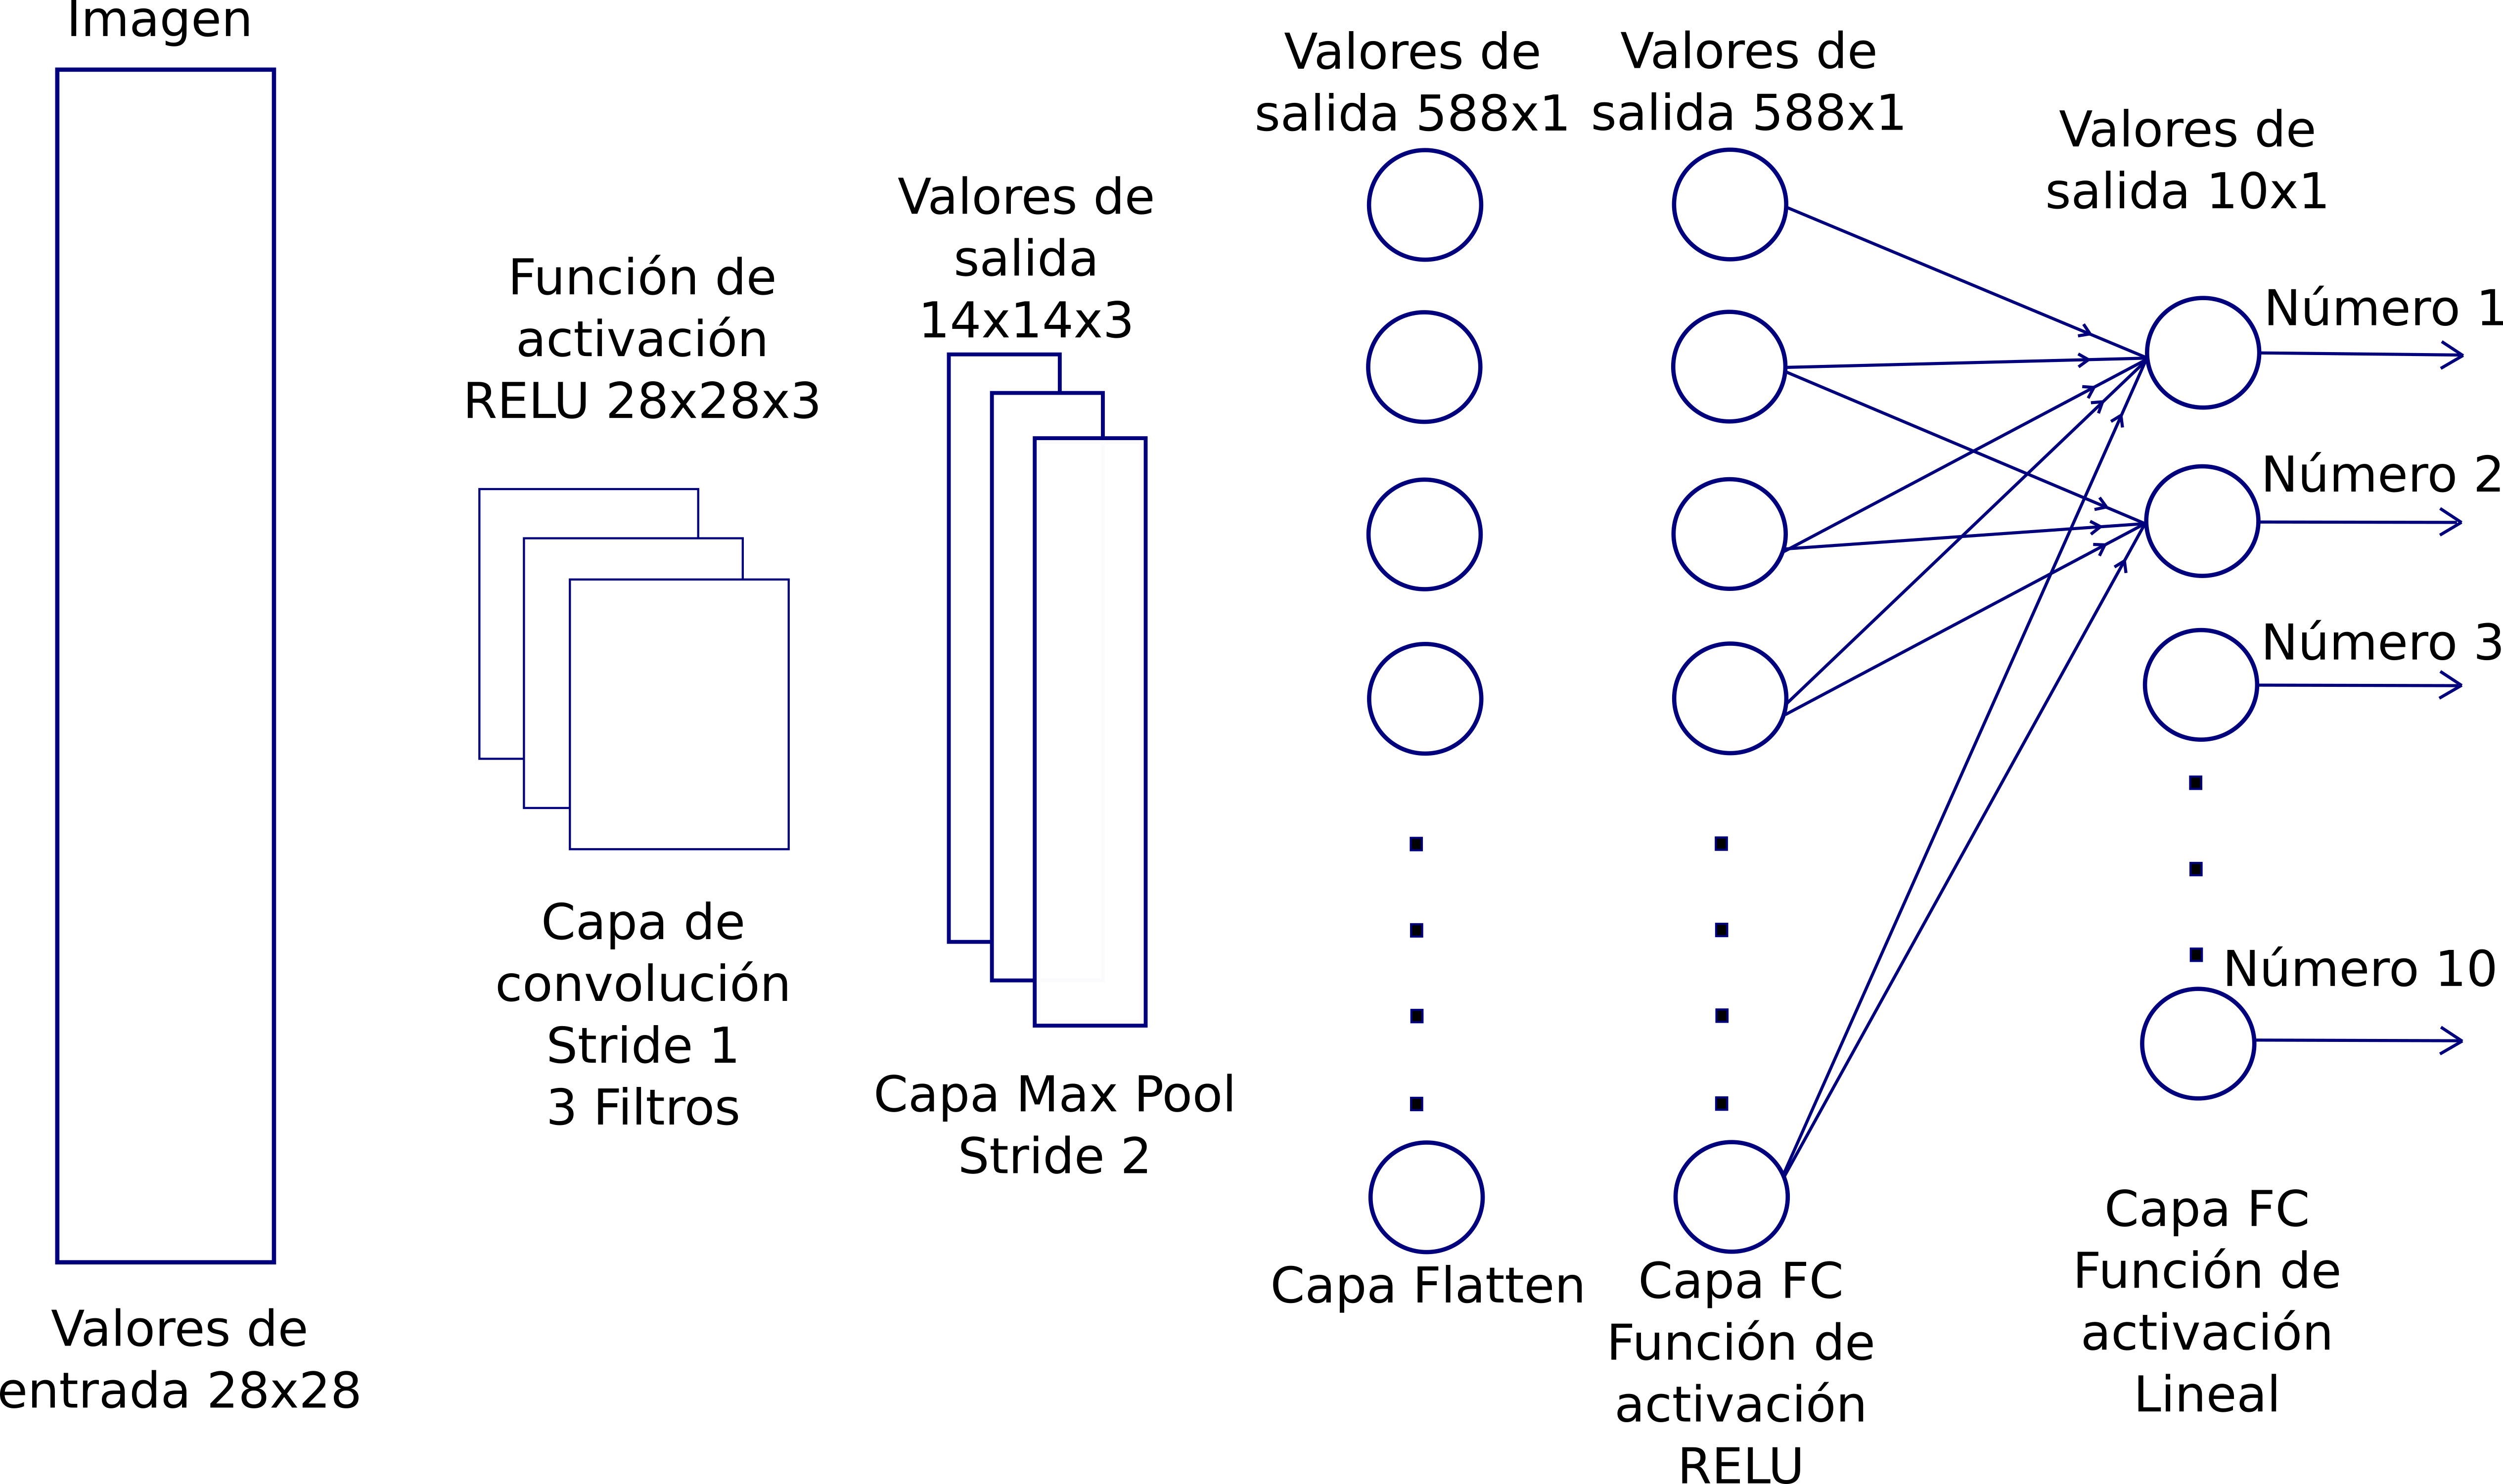
\includegraphics[scale=0.7]{ArquitecturaINK2.png}
\end{center}
    \caption{Esquema de la arquitectura básica de una CNN. Primero, los 28x28 valores de entrada son utilizados por las neuronas de la capa de convolución, y son creados 3 filtros con la intención de extraer propiedades importantes. Después, se seleccionan los valores más grandes con la capa Max Pool para un cierto tamaño de kernel. Posteriormente, se aplanan los valores en un vector de dimensión 588x1 para que sirvan como valores de entrada para una capa densa. Finalmente, se calculan los números a los que corresponde cada imagen.}
    \label{fig:ES-CN}
\end{figure}
Esta misma arquitectura se utilizó como base para construir los modelos convolucionales. Como podemos ver, están conformadas de la siguiente manera: primero, se utiliza las intensidades de una imagen inicial como valores de entrada; en seguida, una capa convolucional realiza la creación de filtros que intentan extraer características importantes de las imágenes, como son por ejemplo grandientes de intensidad, curvas o lineas; en tercer lugar, se realiza de nuevo una selección de los valores más importantes para el análisis en cada filtro; en cuarto lugar, se aplanan o alinean los valores obtenidos por las capas anteriores para utilizarlos como datos iniciales en una capa densa; finalmente, se aplica una capa densa con una función de activación lineal para obtener los logits de la probabilidad de la clase que se busca predecir.
\begin{figure}[H]
    \centering
    \begin{subfigure}[c]{0.4\textwidth}
        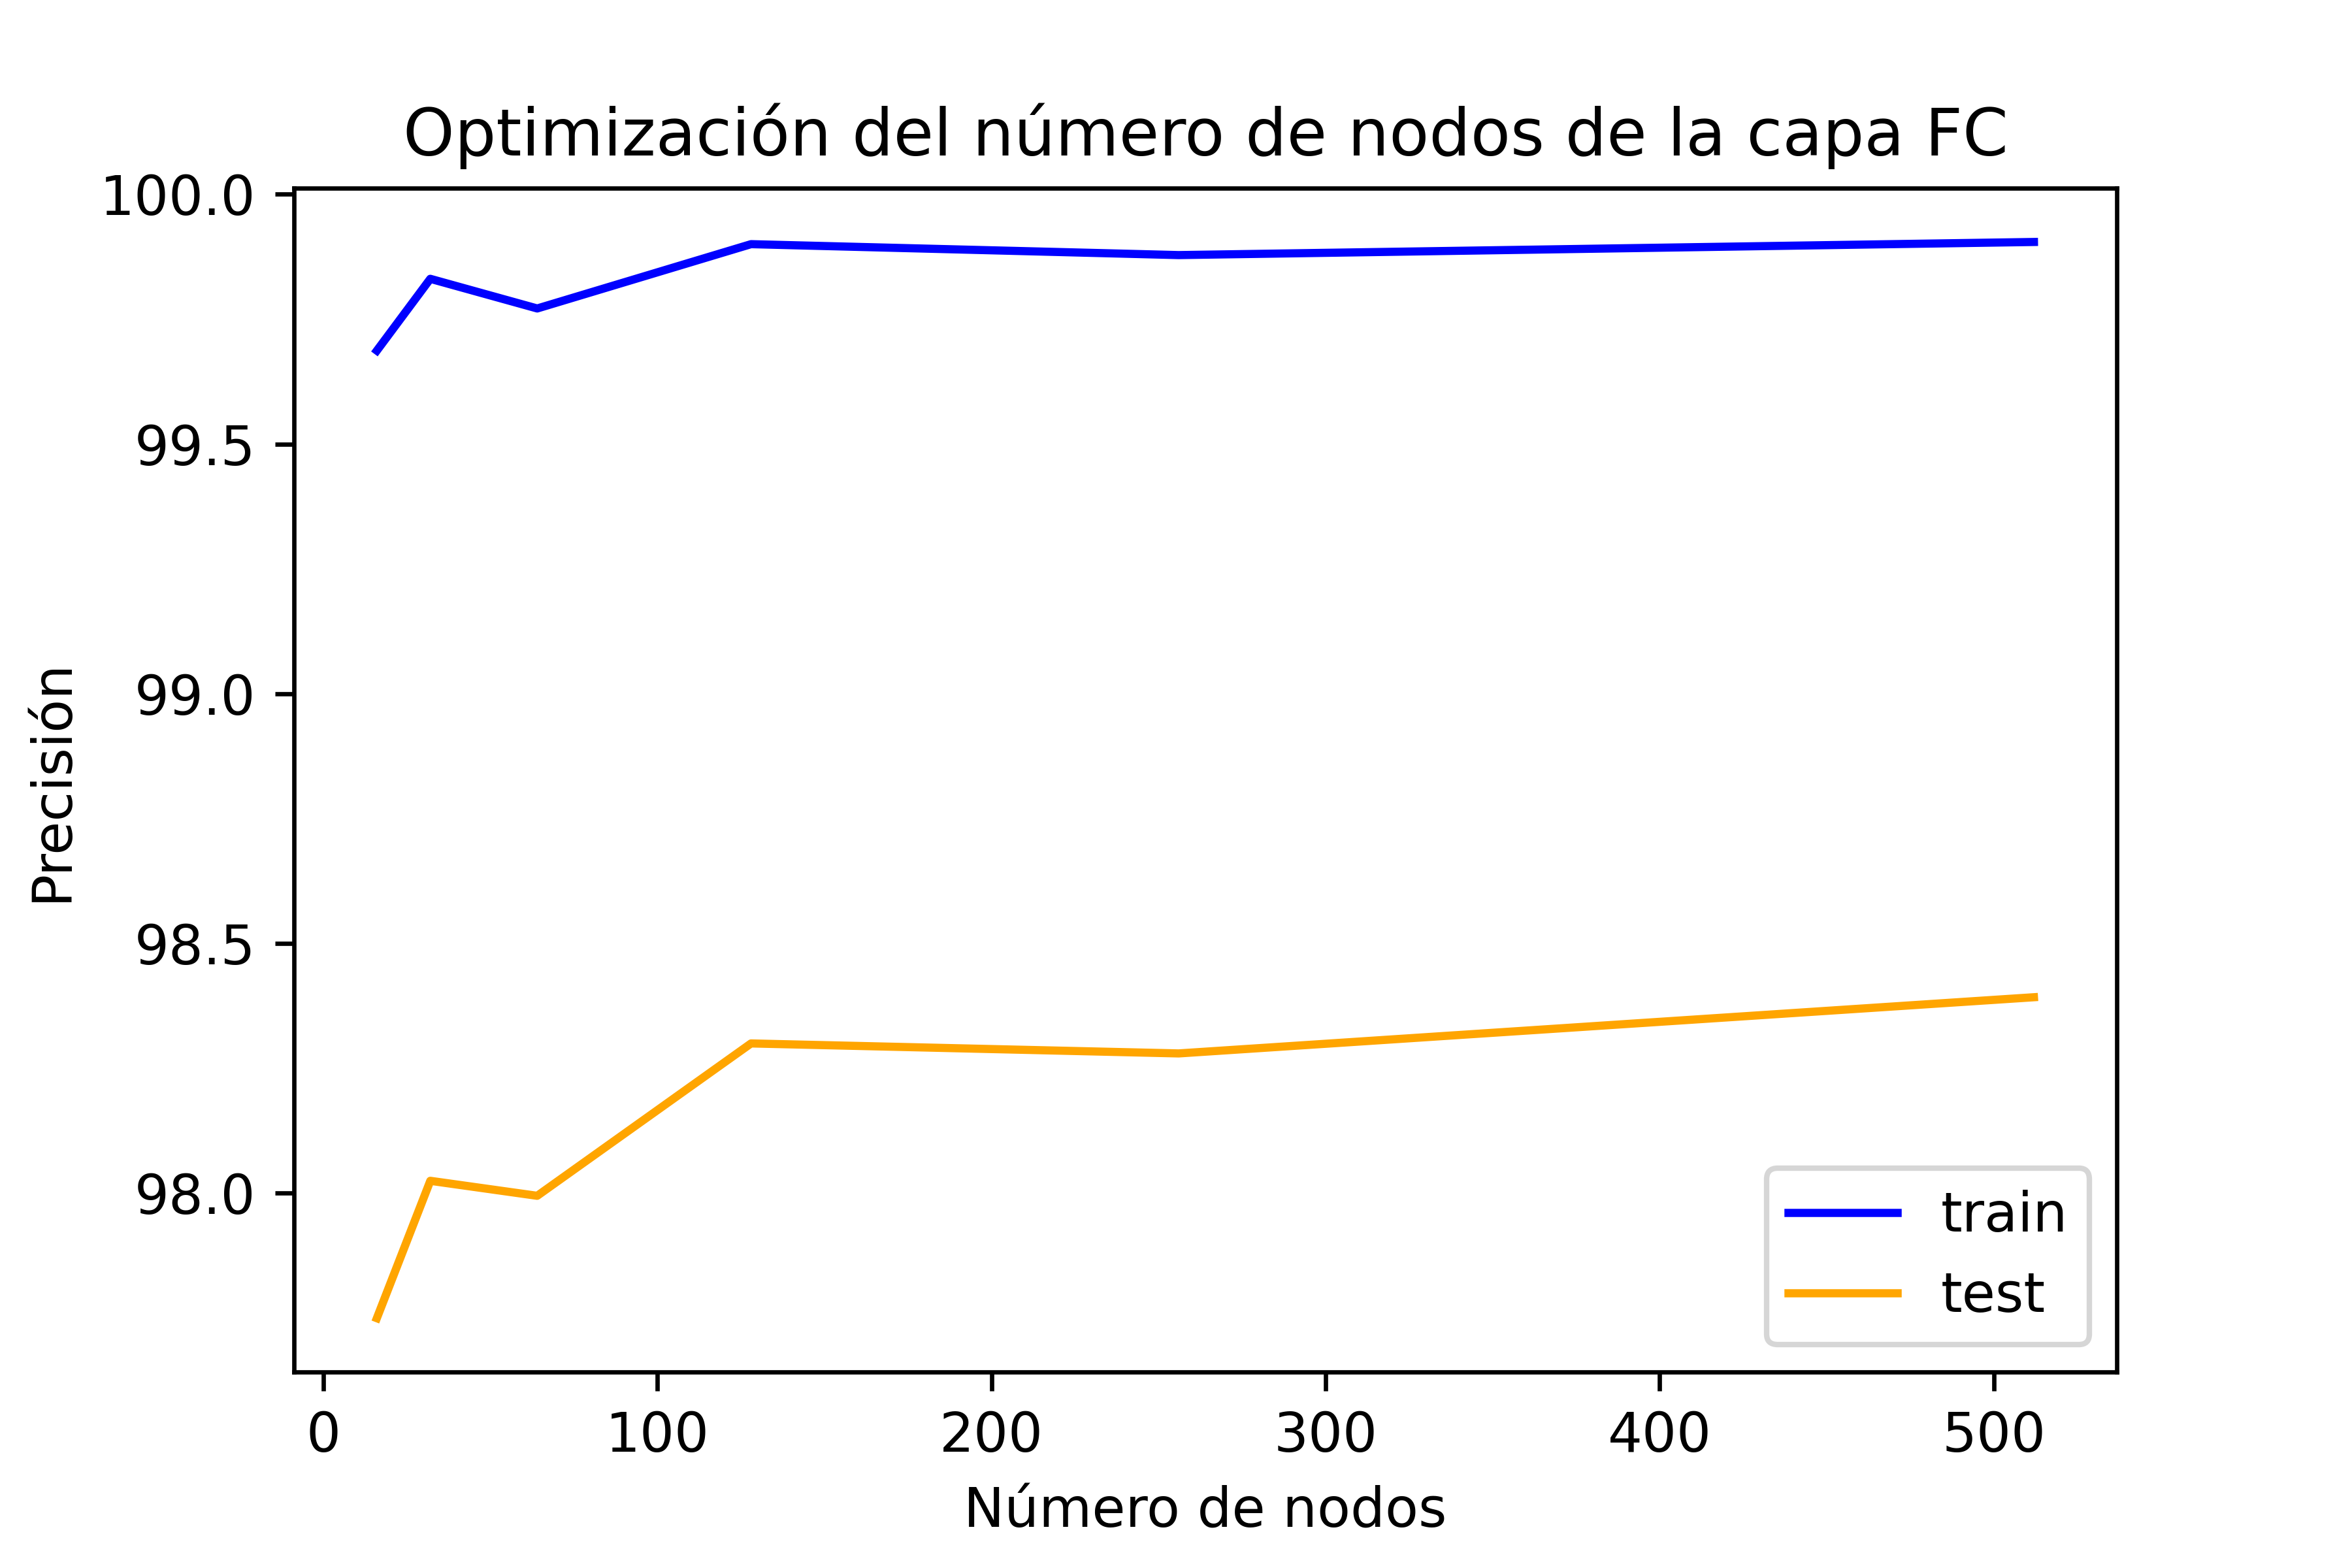
\includegraphics[width=\textwidth]{FCNodes.png}
        \caption{}
        \label{fig:FCNodes}
    \end{subfigure}
    \begin{subfigure}[c]{0.4\textwidth}
        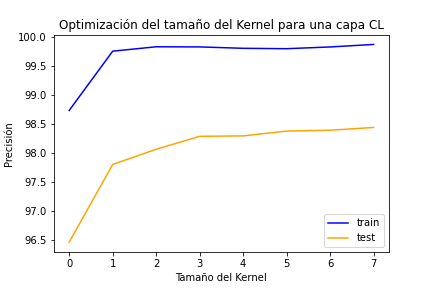
\includegraphics[width=\textwidth]{KernelSize.png}
        \caption{}
        \label{fig:KernelSize}
    \end{subfigure}
    \begin{subfigure}[c]{0.4\textwidth}
        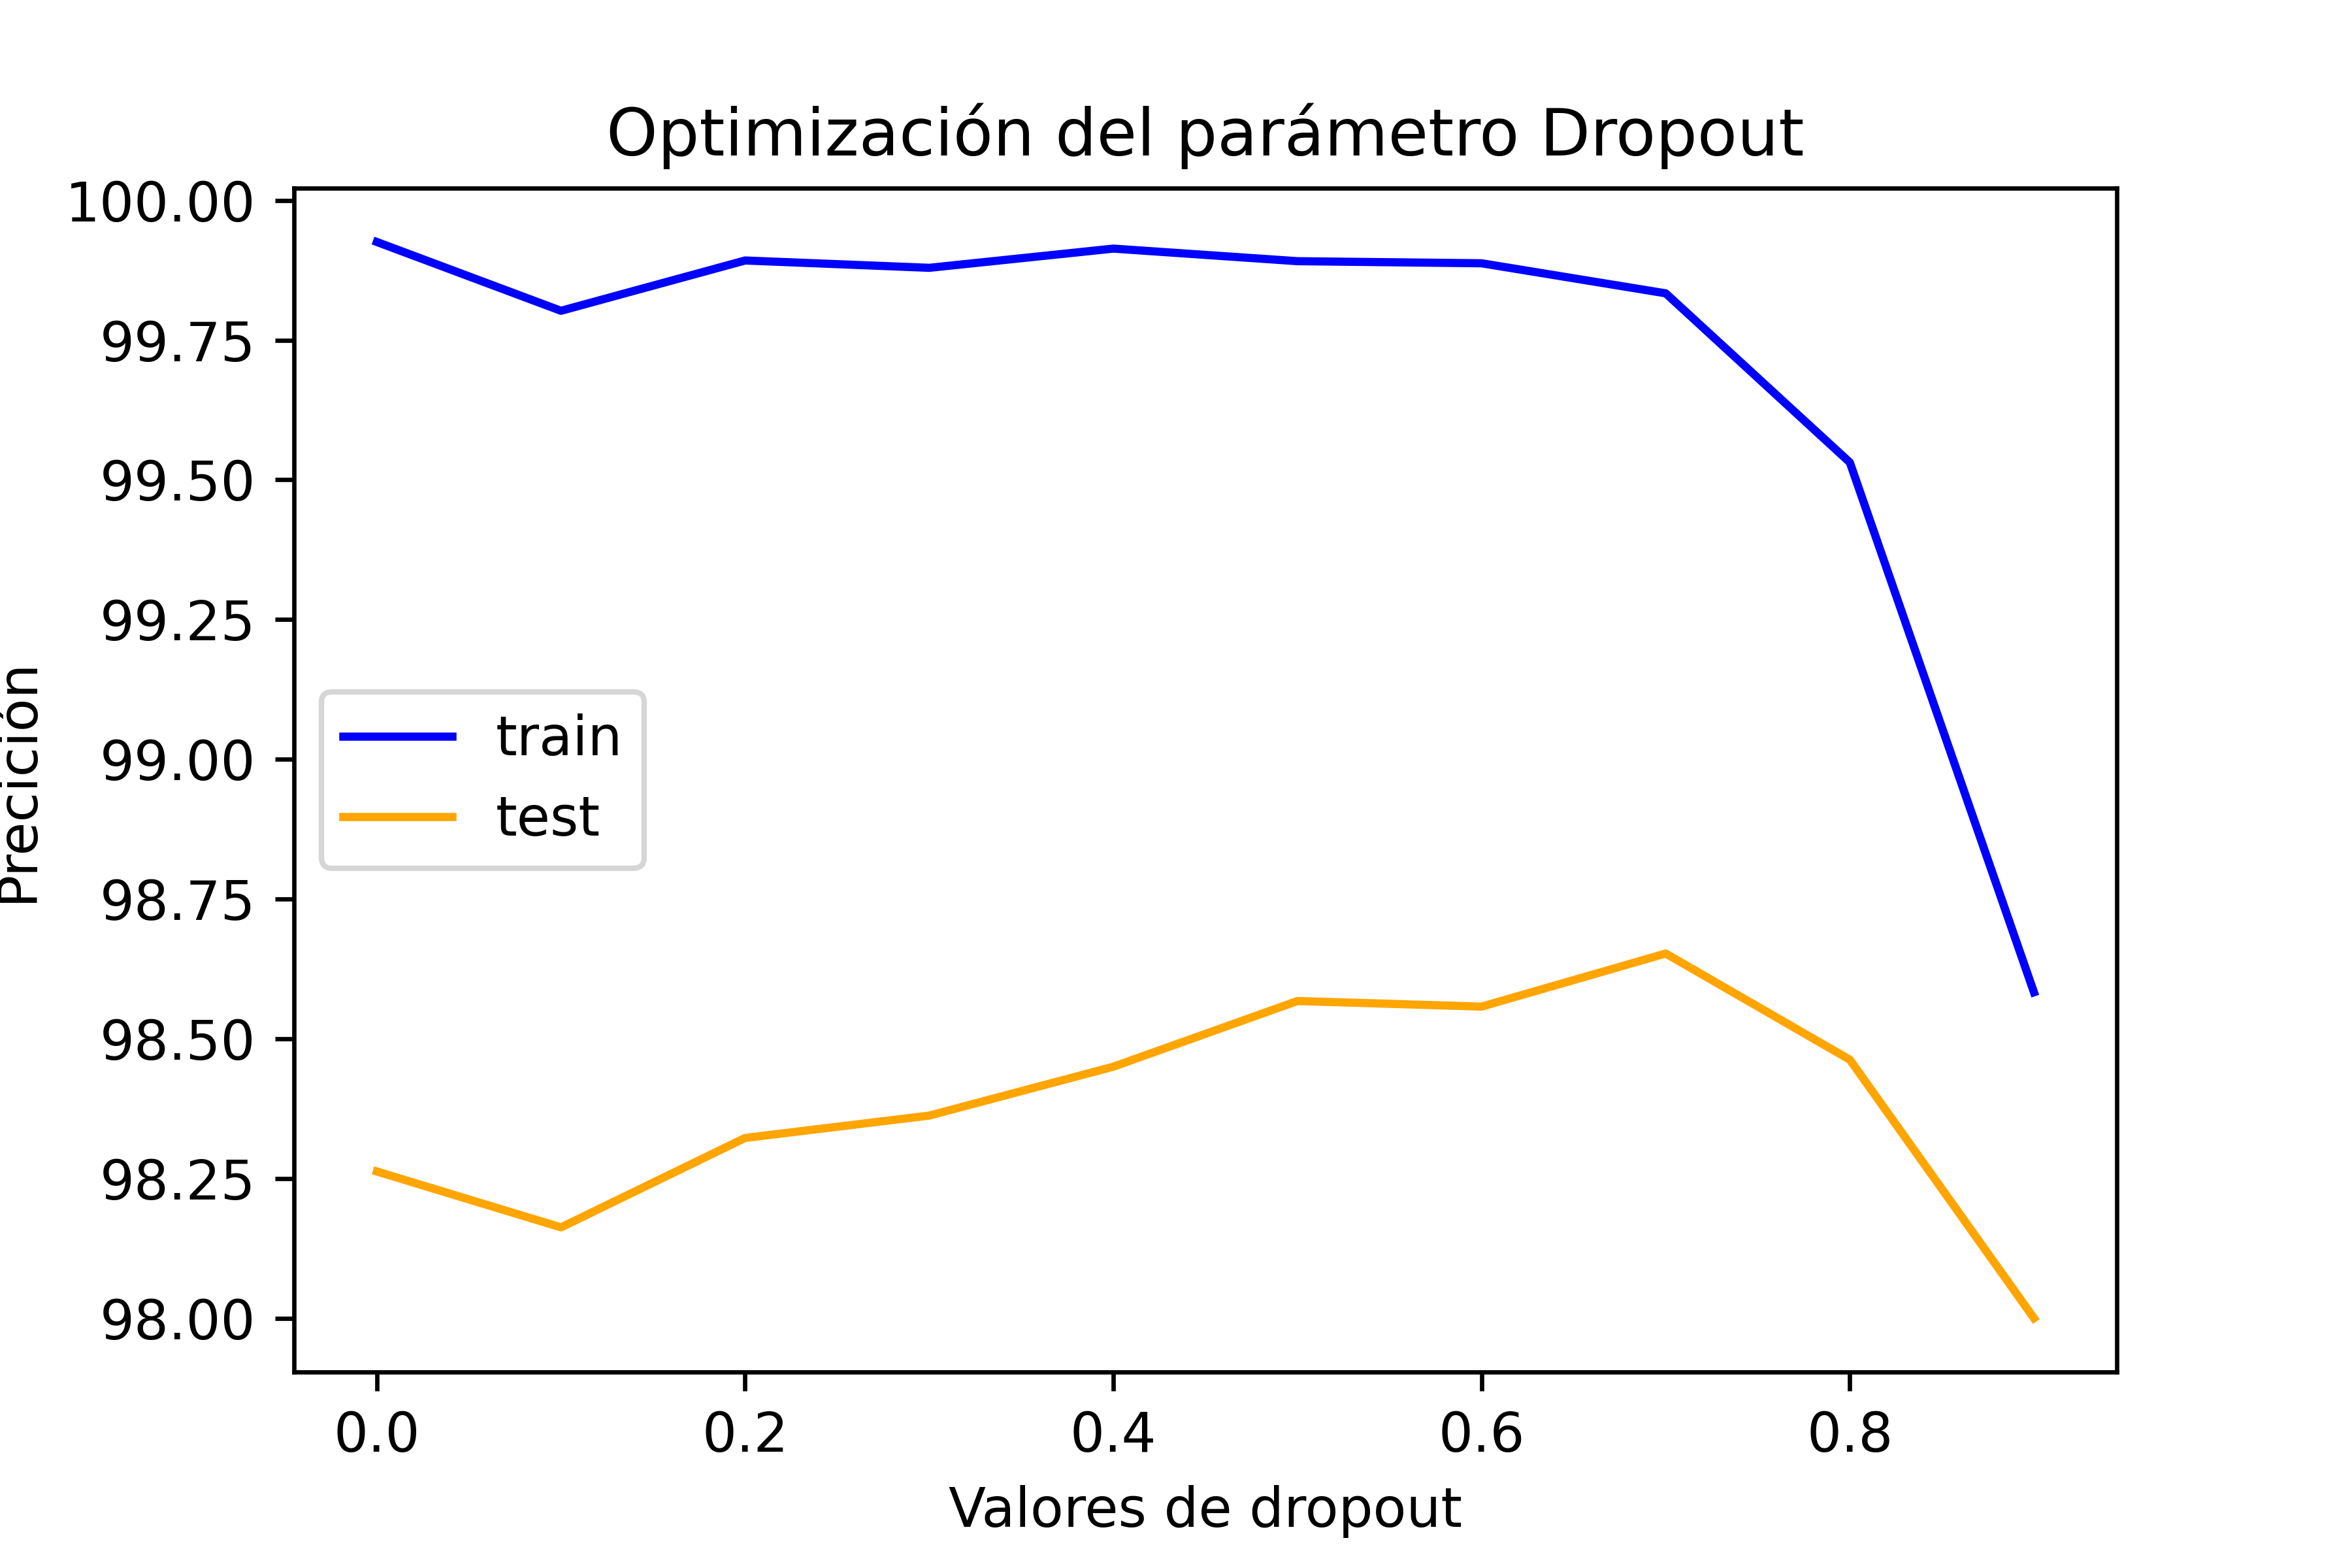
\includegraphics[width=\textwidth]{DropOut.png}
        \caption{}
        \label{fig:DropOut}
    \end{subfigure}
    \begin{subfigure}[c]{0.4\textwidth}
        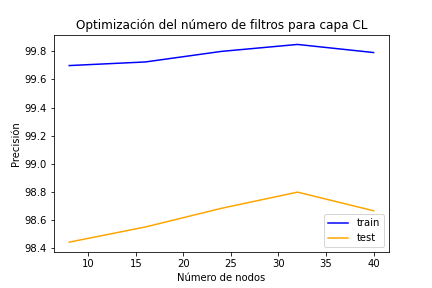
\includegraphics[width=\textwidth]{ConvolutinoNodes.png}
        \caption{}
        \label{fig:ConvNodes}
    \end{subfigure}
    \begin{subfigure}[c]{0.4\textwidth}
        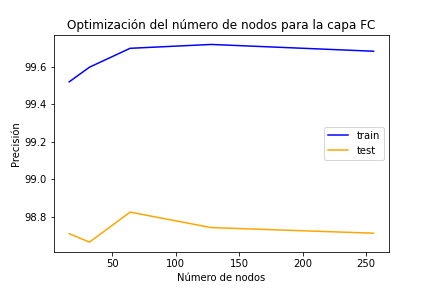
\includegraphics[width=\textwidth]{FullConnectedNodes-2CL.png}
        \caption{}
        \label{fig:FullConn2CL}
    \end{subfigure}
    \begin{subfigure}[c]{0.4\textwidth}
        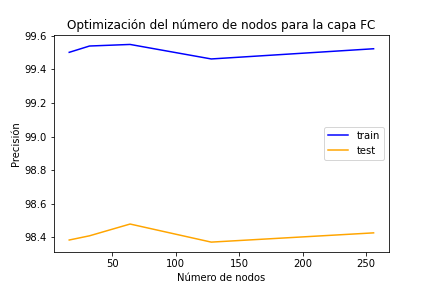
\includegraphics[width=\textwidth]{FullConnectedNodes-3CL.png}
        \caption{}
        \label{fig:FullConn3CL}
    \end{subfigure}
    \caption{Gráficas de diagnóstico para los hiperparámetros de las CNN. Se calcula la precisión para diferentes: a) números de nodos de la capa dense del CNN1; b) tamaños del kernel del CNN1; c) valores de dropout del CNN2; d) número de filtros del CNN3; e) número de nodos de la capa dense del CNN4, f) número de nodos de la capa dense del CNN5.}
    \label{fig:6Graf}
\end{figure}
\section*{Anexo 3: Tablas relevantes}
\begin{table}[H]
    \begin{tabular}{c| p{1.5cm}| p{1.5cm}| p{1.5cm}| p{1.5cm}| p{1.5cm}| p{1.5cm}| p{1.5cm}| p{1.5cm}}
        \toprule
        Name &  error &  val error &  cv val error mean &  cv val error std &   loss &  val loss &  cv val loss mean &  cv val loss std \\
        \midrule
        Log  & 6.0500 &     7.8000 &             7.7650 &            0.1977 & - & - & - & - \\ 
        DNN1 & 1.9350 &     2.3667 &             4.9300 &            0.2563 & 0.0577 &    0.1036 &            0.1586 &           0.0101 \\
        DNN2 & 0.0000 &     2.4444 &             2.9975 &            0.3816 & 0.0000 &    0.3416 &            0.6622 &           0.1558 \\
        DNN3 & 0.9725 &     2.6333 &             3.3800 &            0.1691 & 0.0331 &    0.1929 &            0.1605 &           0.0131 \\
        DNN4 & 1.3425 &     2.6222 &             8.4700 &            0.5439 & 0.3547 &    0.3901 &            1.3511 &           0.0499 \\
        DNN5 & 1.1525 &     2.5444 &             8.0775 &            0.6088 & 0.3680 &    0.4323 &            1.3359 &           0.0314 \\
        DNN6 & 1.0500 &     2.5333 &             8.0550 &            0.8987 & 0.3582 &    0.4060 &            1.3664 &           0.0401 \\
        CNN1 & 0.0000 &     1.6556 &             2.6675 &            0.1904 & 0.0000 &    0.1768 &            0.2766 &           0.0314 \\
        CNN2 & 0.2875 &     1.7667 &             2.1700 &            0.3061 & 0.0098 &    0.1243 &            0.1127 &           0.0187 \\
        CNN3 & 0.0000 &     1.1222 &             1.7900 &            0.0987 & 0.0000 &    0.0857 &            0.2167 &           0.0825 \\
        CNN4 & 0.2575 &     0.8889 &             0.9050 &            0.1171 & 0.0078 &    0.0478 &            0.0535 &           0.0138 \\
        CNN5 & 0.1600 &     0.7222 &             0.9000 &            0.1951 & 0.0051 &    0.0458 &            0.0612 &           0.0153 \\
        CNN6 & 1.7055 &     0.7889 &             0.6950 &            0.0911 & 0.0553 &    0.0313 &            0.0237 &           0.0051 \\
        \bottomrule
        \end{tabular}
        \caption{Estadísticas de pérdida para los modelos. El modelo ``Log'' corresponde a la regresión logística. Las tasas de error están presentadas en porcentaje}
    \label{tab:fullErrors}
\end{table}
\begin{table}[H]
    \centering
    \begin{tabular}{c| p{1.5cm}| p{1.5cm}| p{2cm}| p{1.5cm}}
        \toprule
        Name &  Trainable Parameters &  Dense Layers &  Convolution Layers &  execution  time (hours) \\
        \midrule
        Log & 7850 & - & - & 13.2 \\
        DNN1 &                318010 &             1 &                   0 &                   0.7020 \\
        DNN2 &                178110 &             2 &                   0 &                   0.7002 \\
        DNN3 &                178110 &             2 &                   0 &                   0.7146 \\
        DNN4 &                188210 &             3 &                   0 &                   0.7586 \\
        DNN5 &                203260 &             3 &                   0 &                   0.7545 \\
        DNN6 &                213360 &             4 &                   0 &                   0.7988 \\
        CNN1 &                542230 &             1 &                   1 &                   0.4366 \\
        CNN2 &                542230 &             1 &                   1 &                   0.4467 \\
        CNN3 &                179926 &             1 &                   2 &                   0.4867 \\
        CNN4 &                180118 &             1 &                   2 &                   0.5449 \\
        CNN5 &                209430 &             1 &                   3 &                   0.6473 \\
        CNN6 &                209430 &             1 &                   3 &                   0.9363 \\
        \bottomrule
    \end{tabular}        
    \caption{Descripción sintetizados de los modelos de redes neuronales}
    \label{tab:fullDescrip}
\end{table}
\begin{table}[h]
    \centering
    \begin{tabular}{lrrrr}
    \toprule
    Conjunto &     error &  val error &  cv val error mean &  cv val error std \\
    \midrule
    Clase 0 &  0.0000 &   0.0000 &           0.1826 &          0.0032 \\
    Clase 1 &  0.0223 &   0.6869 &           0.8696 &          0.0154 \\
    Clase 2 &  0.0000 &   0.6593 &           0.8420 &          0.0149 \\
    Clase 3 &  0.0000 &   0.8483 &           1.0310 &          0.0182 \\
    Clase 4 &  0.0255 &   0.8018 &           0.9845 &          0.0175 \\
    Clase 5 &  0.0549 &   0.8696 &           1.0522 &          0.0186 \\
    Clase 6 &  0.0254 &   0.4429 &           0.6256 &          0.0111 \\
    Clase 7 &  0.0481 &   1.0822 &           1.2649 &          0.0224 \\
    Clase 8 &  0.0259 &   1.1312 &           1.3138 &          0.0233 \\
    Clase 9 &  0.0000 &   0.7067 &           0.8893 &          0.0157 \\
    Global & 0.1600 &     0.7222 &             0.9000 &            0.1951 \\
    \bottomrule
    \end{tabular}
    \caption{Errores por clase y global para el conjunto de entrenamiento, prueba y para validación cruzada del modelo CNN5}
    \label{tab:classError}
\end{table}
\section*{Anexo 4: Figuras relevantes}
\figura{modelsGrid.pdf}{Error de entrenamiento y validación como función de la época para los doce modelos entrenamos. Los modelos CNN fueron entrenados por 50 épocas mientras que los de DNN fueron entrenados por 100}{width = \textwidth}
\figura{crossValGrid.pdf}{Error de entrenamiento y validación para la versión principal como para las 10 iteraciones por Cross Validation para el modelo CNN5}{width = \textwidth}
\figura{crossValCompar.pdf}{Error de entrenamiento y validación para la versión principal como y las promediadas obtenidas por Cross Validation para el modelo CNN5}{width = \textwidth}
\figura{confussionMatTrain.pdf}{Matriz de confusión evaluada sobre el conjunto de prueba para el modelo DNN5}{width = \textwidth}
\figura{predictionExample.pdf}{Ejemplo de un valor mal predicho por el modelo CNN5}{width = 0.8\textwidth}
\pagebreak
\begin{figure}[H]
    \centering
    \begin{subfigure}[c]{0.24\textwidth}
        \centering
        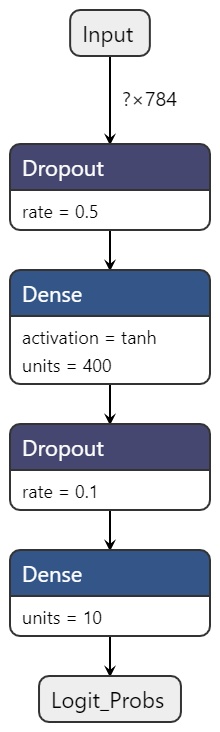
\includegraphics[width = \textwidth]{normal1.png}
        \caption{}
        \label{fig:DNN1}
    \end{subfigure}
    \begin{subfigure}[c]{0.24\textwidth}
        \centering
        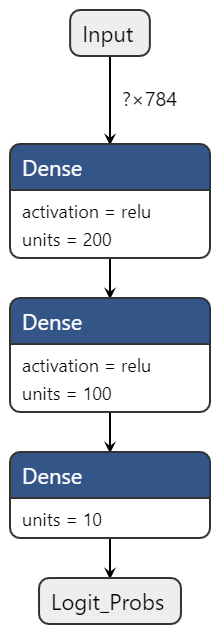
\includegraphics[width = \textwidth]{normal2.png}
        \caption{}
        \label{fig:DNN2}
    \end{subfigure}
    \centering
    \begin{subfigure}[c]{0.24\textwidth}
        \centering
        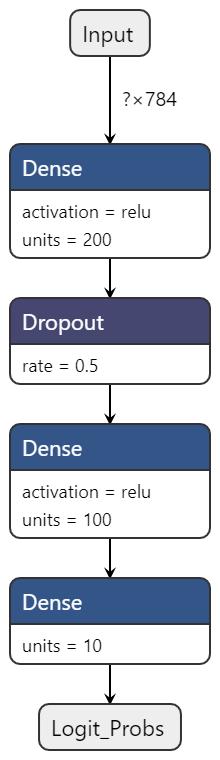
\includegraphics[width = \textwidth]{normal3.png}
        \caption{}
        \label{fig:DNN3}
    \end{subfigure}
    \begin{subfigure}[c]{0.24\textwidth}
        \centering
        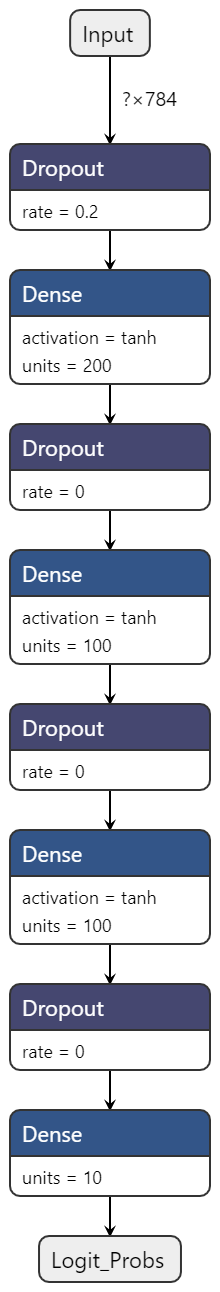
\includegraphics[height = 0.95\textheight]{normal4.png}
        \caption{}
        \label{fig:DNN4}
    \end{subfigure}
    \caption{Diagrama esquemático de los primeros cuatro modelos: (a) normal1, (b) normal2, (c) normal3 y (d) normal4}
\end{figure}
\pagebreak
\begin{figure}[H]
    \centering
    \begin{subfigure}[c]{0.24\textwidth}
        \centering
        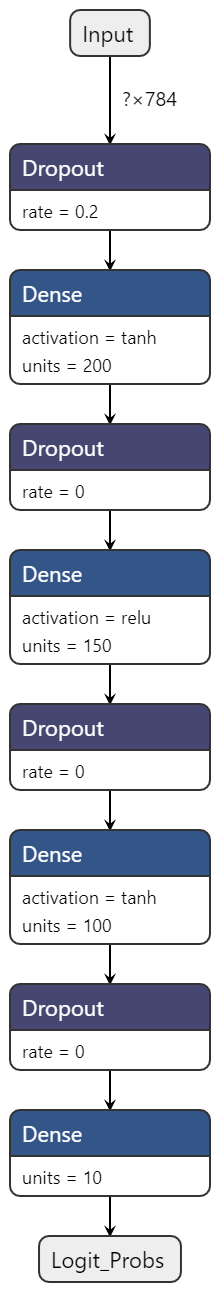
\includegraphics[height = 0.95\textheight]{normal5.png}
        \caption{}
        \label{fig:DNN5}
    \end{subfigure}
    \begin{subfigure}[c]{0.24\textwidth}
        \centering
        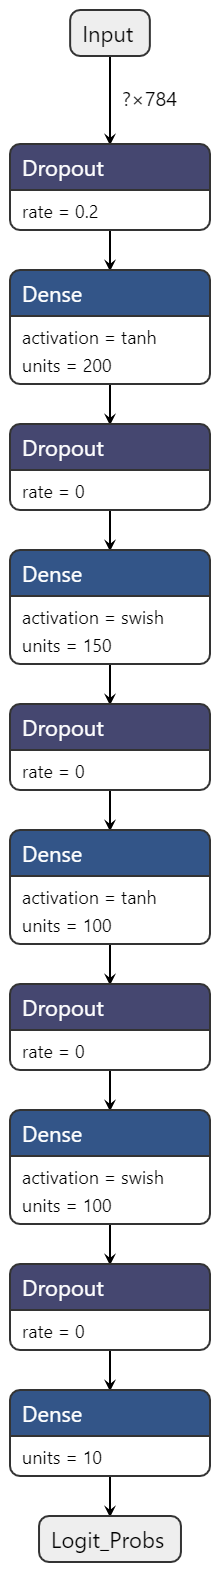
\includegraphics[height = 0.95\textheight]{normal6.png}
        \caption{}
        \label{fig:DNN6}
    \end{subfigure}
    \centering
    \begin{subfigure}[c]{0.24\textwidth}
        \centering
        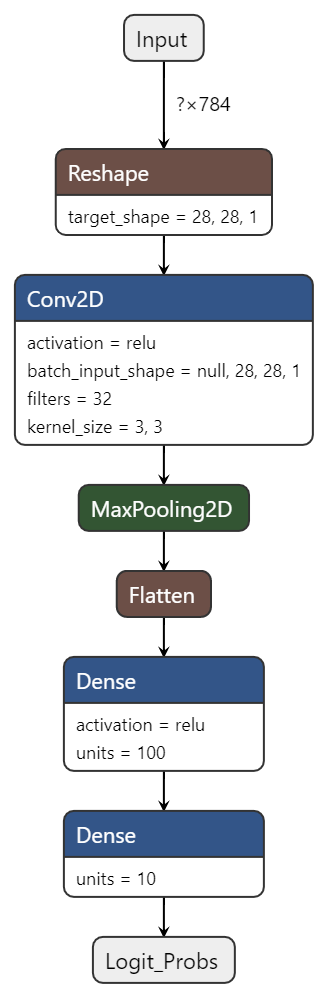
\includegraphics[width = \textwidth]{conv1.png}
        \caption{}
        \label{fig:CNN1}
    \end{subfigure}
    \begin{subfigure}[c]{0.24\textwidth}
        \centering
        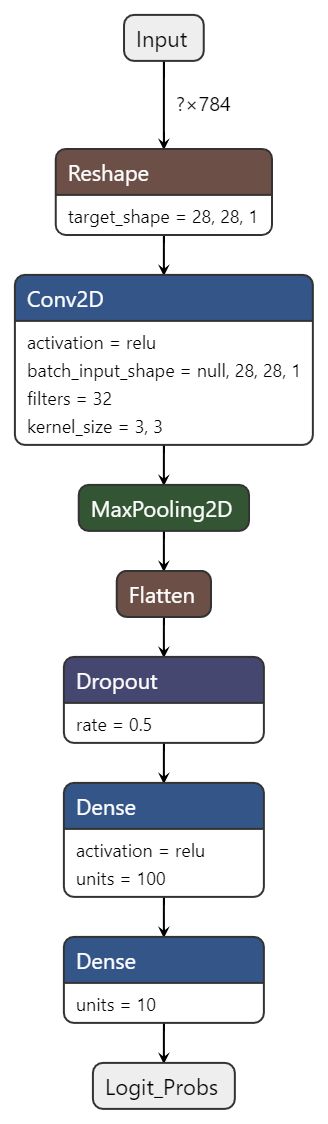
\includegraphics[width = \textwidth]{conv2.png}
        \caption{}
        \label{fig:CNN2}
    \end{subfigure}
    \caption{Diagrama esquemático de los primeros cuatro modelos: (a) normal5, (b) normal6, (c) conv1 y (d) conv2}
\end{figure}
\pagebreak
\begin{figure}[H]
    \centering
    \begin{subfigure}[c]{0.24\textwidth}
        \centering
        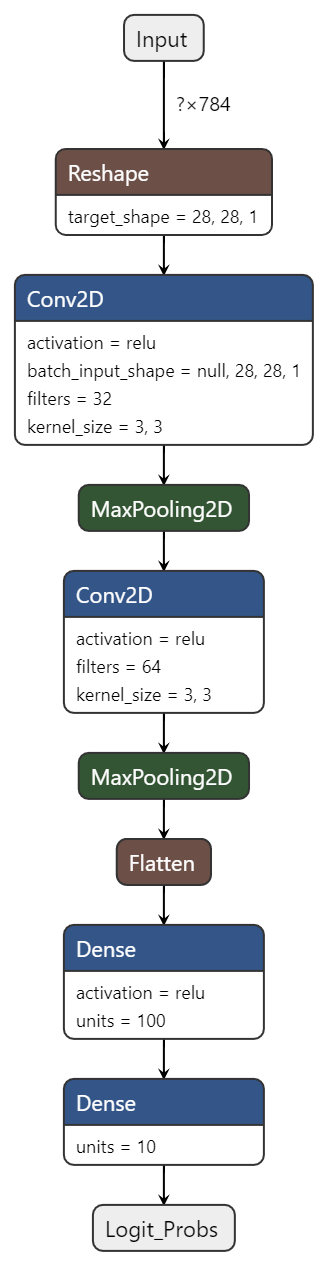
\includegraphics[width = \textwidth]{conv3.png}
        \caption{}
        \label{fig:CNN3}
    \end{subfigure}
    \begin{subfigure}[c]{0.24\textwidth}
        \centering
        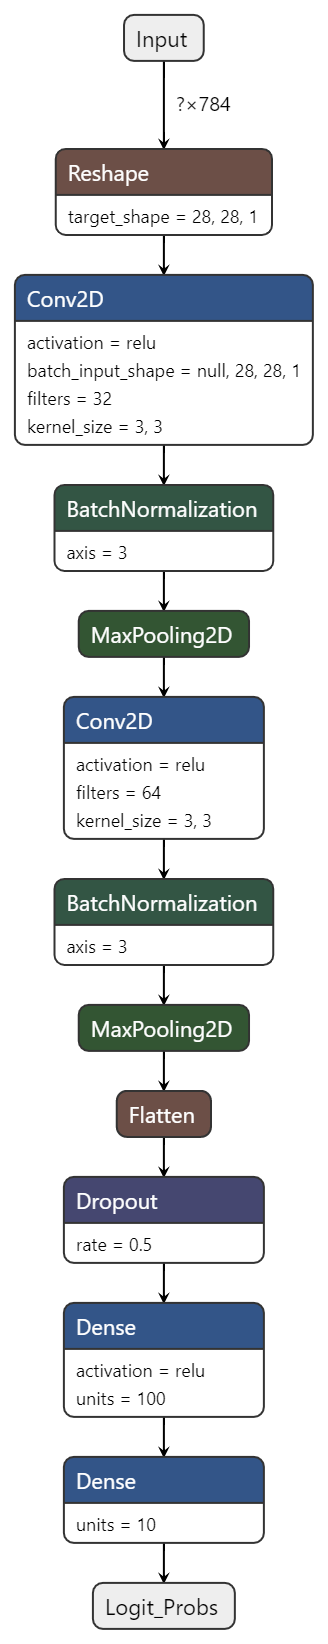
\includegraphics[width = \textwidth]{conv4.png}
        \caption{}
        \label{fig:CNN4}
    \end{subfigure}
    \centering
    \begin{subfigure}[c]{0.24\textwidth}
        \centering
        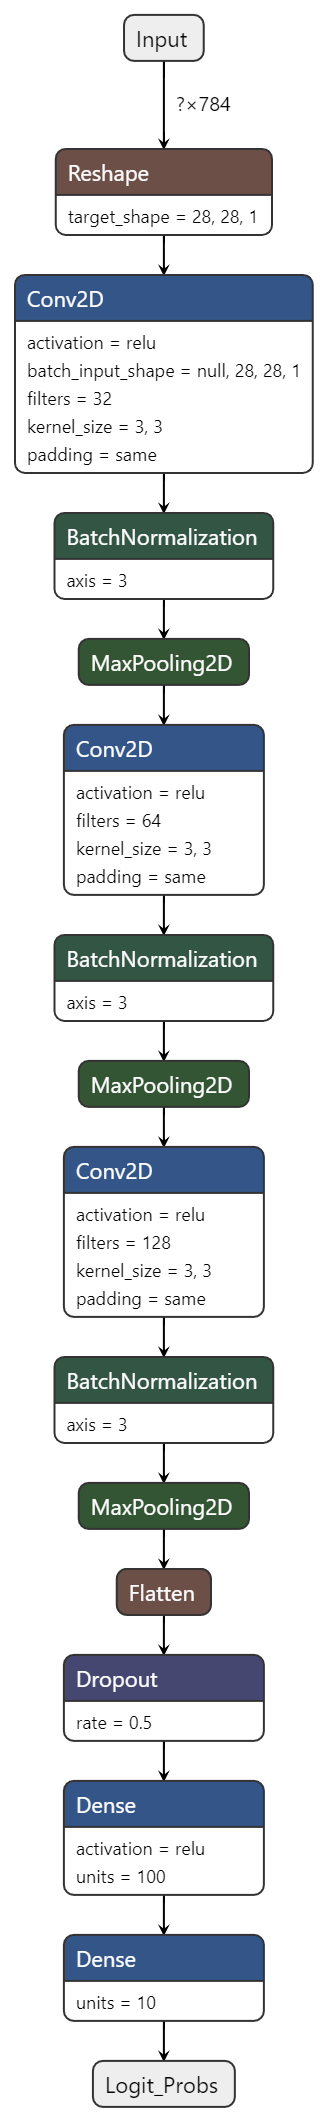
\includegraphics[height =  0.95\textheight]{conv5.png}
        \caption{}
        \label{fig:CNN5}
    \end{subfigure}
    \begin{subfigure}[c]{0.24\textwidth}
        \centering
        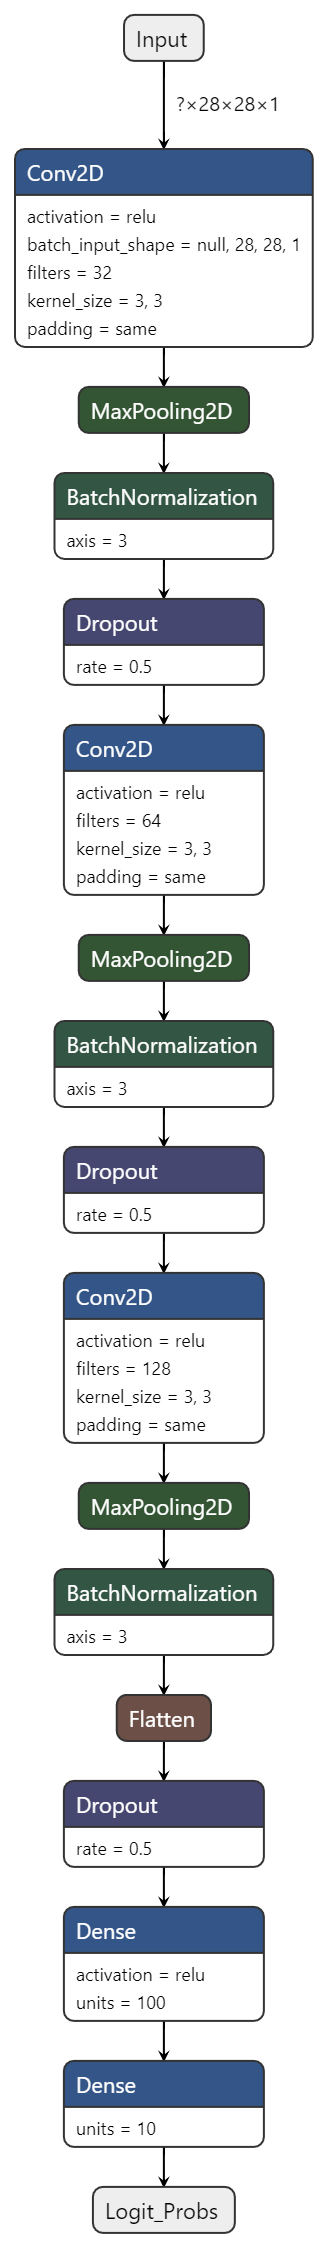
\includegraphics[height =  0.95\textheight]{conv6.png}
        \caption{}
        \label{fig:CNN6}
    \end{subfigure}
    \caption{Diagrama esquemático de los primeros cuatro modelos: (a) conv3, (b) conv4, (c) conv5 y (d) conv6}
\end{figure}
\pagebreak
\begin{thebibliography}{9}
    \bibitem{lecunn} MNIST Handwritten Digit Data Base. Yann LeCunn, Corina Cortes and Chris Burges. \url{http://yann.lecun.com/exdb/mnist/}. Accesado el 02-06-2020.
    \bibitem{Ripley} Ripley, B. D. \textit{Pattern Recognition and Neural Netowrks}. Primera Edición. Cambridge University Press. 1996.
    \bibitem{Goodfellow} Goodfellow, I; Bengio, Y, y Courville, A. \textit{Deep Learning}. Primera Edición. MIT Press. \url{www.deeplearningbook.org}
    \bibitem{Elements} Hastie, T; Tibshirani, R. y Friednman, J. \textit{The Elements of Statistical Learning}. Segunda Edición. Springer. 2009.
    \bibitem{Efron} Efron, B. y Hastie, T. \textit{Computer Age Statistical Inference}. Primera Edición. Cambridge University Press. 2016.
    \bibitem{tf} Keras Overview | TensorFlow Core. \url{https://www.tensorflow.org/guide/keras}. Accesado el 04-06-2020
\end{thebibliography}
\end{document}
